%%%%%%%%%%%%%%%%%%%%%%%%%%%%%%%%%%%%%%%%%%%%%%%%%%%%%%%%%%%%%%%%%%%%%%%%%%%%%%%%
%2345678901234567890123456789012345678901234567890123456789012345678901234567890
%        1         2         3         4         5         6         7         8

\documentclass[letterpaper, 10 pt, conference]{IEEEtran}  % Comment this line out if you need a4paper

%\documentclass[a4paper, 10pt, conference]{ieeeconf}      % Use this line for a4 paper

\IEEEoverridecommandlockouts                              % This command is only needed if 
                                                          % you want to use the \thanks command

%\overrideIEEEmargins                                      % Needed to meet printer requirements.

\usepackage[T1]{fontenc}
\usepackage[utf8]{inputenc}

\usepackage{tikz}
\usetikzlibrary{calc,patterns,angles,quotes,shapes}

% See the \addtolength command later in the file to balance the column lengths
% on the last page of the document

% The following packages can be found on http:\\www.ctan.org
\usepackage{graphics} % for pdf, bitmapped graphics files
\usepackage{epsfig} % for postscript graphics files
\usepackage{mathptmx} % assumes new font selection scheme installed
\usepackage{times} % assumes new font selection scheme installed
\usepackage{amsmath} % assumes amsmath package installed
\usepackage{amssymb}  % assumes amsmath package installed


\title{\LARGE \bf
    The TransHumUs project for the French Pavilion \\ at La Biennale di Venezia 2015
}


%\author{Albert Author$^{1}$ and Bernard D. Researcher$^{2}$% <-this % stops a space
%\thanks{*This work was not supported by any organization}% <-this % stops a space
%\thanks{$^{1}$Albert Author is with Faculty of Electrical Engineering, Mathematics and Computer Science,
        %University of Twente, 7500 AE Enschede, The Netherlands
        %{\tt\small albert.author@papercept.net}}%
%\thanks{$^{2}$Bernard D. Researcheris with the Department of Electrical Engineering, Wright State University,
        %Dayton, OH 45435, USA
        %{\tt\small b.d.researcher@ieee.org}}%
%}


\begin{document}



\maketitle
\thispagestyle{empty}
\pagestyle{empty}


%%%%%%%%%%%%%%%%%%%%%%%%%%%%%%%%%%%%%%%%%%%%%%%%%%%%%%%%%%%%%%%%%%%%%%%%%%%%%%%%
\begin{abstract}
    TODO
\end{abstract}
%%%%%%%%%%%%%%%%%%%%%%%%%%%%%%%%%%%%%%%%%%%%%%%%%%%%%%%%%%%%%%%%%%%%%%%%%%%%%%%%
\section{When robotics meets art}
\subsection{The transHumUs project of Céleste Boursier-Mougenot}

\begin{figure}[thpb]
    \centering
    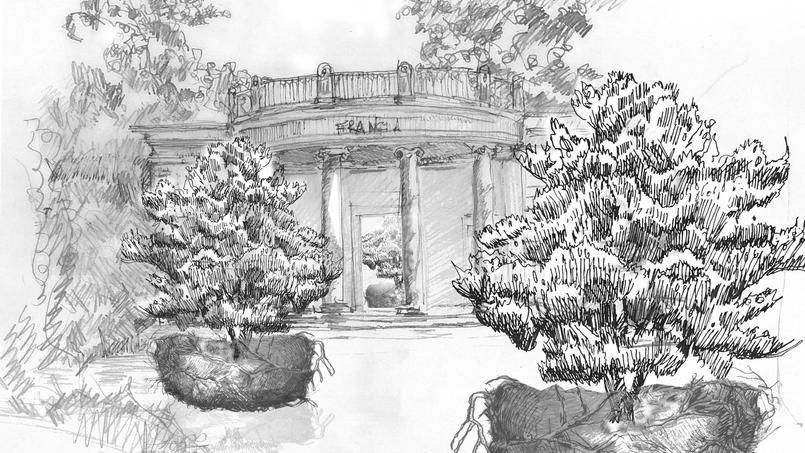
\includegraphics[width=\linewidth]{img/vue_artiste.jpg}
    \caption{Artist's Impression}
    \label{artists_impression}
\end{figure}

For the 56th edition of the Venice Biennale International Contemporary Art Exhibit, Céleste Boursier-Mougenot composed a poetic work evoking the follies of 18th-century romantic parks, while revealing its political dimension.

With rêvolutions by artist Céleste Boursier-Mougenot, accompanied by the exhibit’s Curator, Emma Lavigne, the French Pavilion of the Venice Biennale has been transformed into an organic, dreamlike isle.

Under the glass roof, with the Pavilion’s flight and tree-lined lanes of the Giardini, Céleste Boursier-Mougenot has rolled out the choreography of three mobile trees moving according to their metabolism, the varying flow of their sap and their sensitivity when going from shadow to light.

\subsection{The robotics interpretation}

TODO interpretation → discours sur le mouvement

\section{The robotic project}
\subsection{Specifications}

Acording to the artist's wishes, we established the initial specifications for the piece of art, in order to find the right industrial partners:

\begin{itemize}
    \item The artwork will be composed by three trees of approximately 4 to 5 meters high and 3 tons;
    \item They will move in accordance with some feedback from their metabolism;
    \item The movement will be holonomic in a plane;
    \item The trees will have to move silently;
    \item The motion must be really slow, hardly perceptible (between 0 and 1 meter per minute);
    \item The trajectory shall cover as much as possible the available space;
    \item Several trees will have to coordinate themselves in the same area;
    \item The wheelbase must be able to roll on soft floors (mud and gravels) as well as on hard ones (concrete).
\end{itemize}

\subsection{Technical solutions}

\paragraph{Sapflow sensors} have been selected by biology researchers as they can provide a reliable signal correlated with the tree's metabolism.

\paragraph{Automatic Guided Vehicles} (AGV) with three directable wheels should comply with the admissible mechanical load on the concrete and provide an overall holonomic motion possibility.

\paragraph{Absolute geolocation} that works well indoor and outdoor, including on bumpy areas, at an affordable price is hard to find, but exists.

\subsection{Architecture for the generation of motion}

As the artist wants an holonomic planar motion, in the most basic form, we need input 3 variables. The artist also wish that the trees behave in a similar manner in whatever direction it goes, so we choose a polar coordinate system concentric with the AGV: $(v, \theta, \omega)$, where:

\begin{itemize}
    \item $\theta \in [0, 2\pi[$ is the direction of the center of the AGV;
    \item $v \in [-1, 1]$ is its linear velocity along the direction $\theta$;
    \item $\omega \in [-1, 1]$ is its angular velocity.
\end{itemize}

With this system, we can easily compute the output needed by the AGV, which consist of the orientation $\theta_i$ of each wheel and its traction velocity $v_i$:

\begin{eqnarray*}
    v_{xi} &=& v \cos(\theta)- \omega \sin(\alpha_i) \\
    v_{yi} &=& v \sin(\theta)+ \omega \cos(\alpha_i) \\
    v_i &=& \sqrt{v_{xi}^2 + v_{yi}^2} \\
    \theta_i &=& \arctan(v_{yi}, v_{xi})
\end{eqnarray*}


\begin{figure}[thpb]
    \centering
    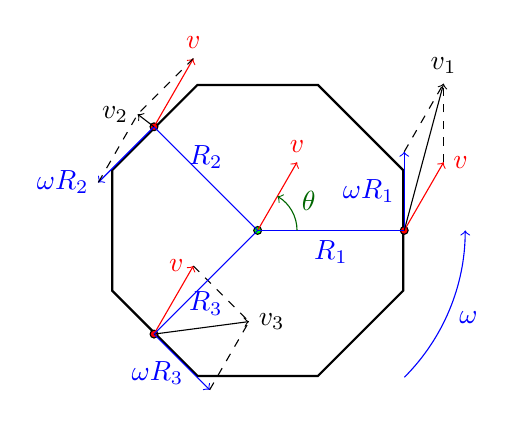
\begin{tikzpicture}
        \coordinate (o) at (0,0);
        \coordinate (v) at (0.5, {sqrt(3) / 2});
        \coordinate (x) at ({-sqrt(2) / 2}, {-sqrt(2) / 2});
        \coordinate (y) at ({+sqrt(2) / 2}, {-sqrt(2) / 2});
        \coordinate (z) at (0, 1);
        \draw (o) node [draw,thick,minimum size=4cm,name=O,regular polygon,regular polygon sides=8] {};
        \draw (O) node [fill=green,circle,draw,inner sep=1pt] {};
        \coordinate (a) at (O.side 2);
        \coordinate (b) at (O.side 4);
        \coordinate (c) at (O.side 7);
        \coordinate (d) at (O.side 6);
        \draw (a) node [fill=red,circle,draw,inner sep=1pt] {};
        \draw (b) node [fill=red,circle,draw,inner sep=1pt] {};
        \draw (c) node [fill=red,circle,draw,inner sep=1pt] {};
        \draw [->, red] (o) -- (v) node [above] {$v$};
        \draw [->, red] (a) -- ++(v) node [above] {$v$};
        \draw [->, red] (b) -- ++(v) node [left] {$v$};
        \draw [->, red] (c) -- ++(v) node [right] {$v$};
        \draw [->, blue] (a) -- ++(x) node [left] {$\omega R_2$};
        \draw [->, blue] (b) -- ++(y) node [pos=0.7, left] {$\omega R_3$};
        \draw [->, blue] (c) -- ++(z) node [pos=0.5, left] {$\omega R_1$};
        \draw [->] (a) -- ($ (a) + (v) + (x) $) node [left] {$v_2$};
        \draw [->] (b) -- ($ (b) + (v) + (y) $) node [right] {$v_3$};
        \draw [->] (c) -- ($ (c) + (v) + (z) $) node [above] {$v_1$};
        \draw [dashed] ($ (a) + (v) $) -- ($ (a) + (v) + (x) $);
        \draw [dashed] ($ (b) + (v) $) -- ($ (b) + (v) + (y) $);
        \draw [dashed] ($ (c) + (v) $) -- ($ (c) + (v) + (z) $);
        \draw [dashed] ($ (a) + (x) $) -- ($ (a) + (v) + (x) $);
        \draw [dashed] ($ (b) + (y) $) -- ($ (b) + (v) + (y) $);
        \draw [dashed] ($ (c) + (z) $) -- ($ (c) + (v) + (z) $);
        \draw [blue] (o) -- (a) node [pos=0.5, above] {$R_2$};
        \draw [blue] (o) -- (b) node [pos=0.5, below] {$R_3$};
        \draw [blue] (o) -- (c) node [pos=0.5, below] {$R_1$};
        \pic [black!60!green, draw, ->, "$\theta$", angle eccentricity=1.5] {angle = c--o--v};
        \pic [blue, draw, ->, "$\omega$", angle eccentricity=1.1, angle radius=75] {angle = d--o--c};
    \end{tikzpicture}
    \caption{$(v_i, \theta_i)$ as a function of $(v, \theta, \omega)$}
    \label{octogon}
\end{figure}

\begin{itemize}
    \item Présentation générale (schéma octogone avec le CIR)
    \item Schéma bloc
    \item captures d’écran du simulateur
\end{itemize}


\section{Implementation}

Photos

\begin{itemize}
    \item sondes granier
    \item AGV désossé
    \item photo de pose des balises dans l’arbre
    \item arbre en acheminement
\end{itemize}


déroulement du projet
jusqu’à l’inauguration de la ministre



%$$
%\alpha + \beta = \chi \eqno{(1)}
%$$

\section{Conclusion}


\addtolength{\textheight}{-12cm}   % This command serves to balance the column lengths
                                  % on the last page of the document manually. It shortens
                                  % the textheight of the last page by a suitable amount.
                                  % This command does not take effect until the next page
                                  % so it should come on the page before the last. Make
                                  % sure that you do not shorten the textheight too much.
\section*{APPENDIX}
\section*{ACKNOWLEDGMENT}
%References are important to the reader; therefore, each citation must be complete and correct. If at all possible, references should be commonly available publications.
%\begin{thebibliography}{99}
%\bibitem{c1} G. O. Young, ÒSynthetic structure of industrial plastics (Book style with paper title and editor),Ó 	in Plastics, 2nd ed. vol. 3, J. Peters, Ed.  New York: McGraw-Hill, 1964, pp. 15Ð64.
%\bibitem{c2} W.-K. Chen, Linear Networks and Systems (Book style).	Belmont, CA: Wadsworth, 1993, pp. 123Ð135.
%\bibitem{c3} H. Poor, An Introduction to Signal Detection and Estimation.   New York: Springer-Verlag, 1985, ch. 4.
%\bibitem{c4} B. Smith, ÒAn approach to graphs of linear forms (Unpublished work style),Ó unpublished.
%\bibitem{c5} E. H. Miller, ÒA note on reflector arrays (Periodical styleÑAccepted for publication),Ó IEEE Trans. Antennas Propagat., to be publised.
%\bibitem{c6} J. Wang, ÒFundamentals of erbium-doped fiber amplifiers arrays (Periodical styleÑSubmitted for publication),Ó IEEE J. Quantum Electron., submitted for publication.
%\bibitem{c7} C. J. Kaufman, Rocky Mountain Research Lab., Boulder, CO, private communication, May 1995.
%\bibitem{c8} Y. Yorozu, M. Hirano, K. Oka, and Y. Tagawa, ÒElectron spectroscopy studies on magneto-optical media and plastic substrate interfaces(Translation Journals style),Ó IEEE Transl. J. Magn.Jpn., vol. 2, Aug. 1987, pp. 740Ð741 [Dig. 9th Annu. Conf. Magnetics Japan, 1982, p. 301].
%\bibitem{c9} M. Young, The Techincal Writers Handbook.  Mill Valley, CA: University Science, 1989.
%\bibitem{c10} J. U. Duncombe, ÒInfrared navigationÑPart I: An assessment of feasibility (Periodical style),Ó IEEE Trans. Electron Devices, vol. ED-11, pp. 34Ð39, Jan. 1959.
%\bibitem{c11} S. Chen, B. Mulgrew, and P. M. Grant, ÒA clustering technique for digital communications channel equalization using radial basis function networks,Ó IEEE Trans. Neural Networks, vol. 4, pp. 570Ð578, July 1993.
%\bibitem{c12} R. W. Lucky, ÒAutomatic equalization for digital communication,Ó Bell Syst. Tech. J., vol. 44, no. 4, pp. 547Ð588, Apr. 1965.
%\bibitem{c13} S. P. Bingulac, ÒOn the compatibility of adaptive controllers (Published Conference Proceedings style),Ó in Proc. 4th Annu. Allerton Conf. Circuits and Systems Theory, New York, 1994, pp. 8Ð16.
%\bibitem{c14} G. R. Faulhaber, ÒDesign of service systems with priority reservation,Ó in Conf. Rec. 1995 IEEE Int. Conf. Communications, pp. 3Ð8.
%\bibitem{c15} W. D. Doyle, ÒMagnetization reversal in films with biaxial anisotropy,Ó in 1987 Proc. INTERMAG Conf., pp. 2.2-1Ð2.2-6.
%\bibitem{c16} G. W. Juette and L. E. Zeffanella, ÒRadio noise currents n short sections on bundle conductors (Presented Conference Paper style),Ó presented at the IEEE Summer power Meeting, Dallas, TX, June 22Ð27, 1990, Paper 90 SM 690-0 PWRS.
%\bibitem{c17} J. G. Kreifeldt, ÒAn analysis of surface-detected EMG as an amplitude-modulated noise,Ó presented at the 1989 Int. Conf. Medicine and Biological Engineering, Chicago, IL.
%\bibitem{c18} J. Williams, ÒNarrow-band analyzer (Thesis or Dissertation style),Ó Ph.D. dissertation, Dept. Elect. Eng., Harvard Univ., Cambridge, MA, 1993. 
%\bibitem{c19} N. Kawasaki, ÒParametric study of thermal and chemical nonequilibrium nozzle flow,Ó M.S. thesis, Dept. Electron. Eng., Osaka Univ., Osaka, Japan, 1993.
%\bibitem{c20} J. P. Wilkinson, ÒNonlinear resonant circuit devices (Patent style),Ó U.S. Patent 3 624 12, July 16, 1990. 
%\end{thebibliography}
\end{document}
